\def\firstcircle{(0,0) circle (1.5cm)}
\def\secondcircle{(0:2cm) circle (1.5cm)}


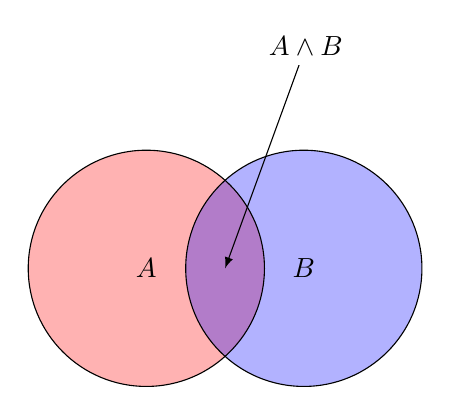
\begin{tikzpicture}
    \begin{scope}[shift={(0cm,0cm)}, fill opacity=0.3]
        \fill[red] \firstcircle;
        \fill[blue] \secondcircle;
    \end{scope}

    \begin{scope}[shift={(0cm,0cm)}]
       \draw \firstcircle node[] {$A$};
        \draw \secondcircle node [] {$B$};
    \end{scope}
\draw[latex-]  (1,0) -- ++ (70:3) node[fill=white] {$A \wedge B$};
\end{tikzpicture}
